\documentclass[conference]{IEEEtran}
% Shared preamble for the five papers (IEEE conference format).
\usepackage[T1]{fontenc}
\usepackage{cite}
\usepackage{amsmath,amssymb,amsfonts}
\usepackage{graphicx}
\usepackage{booktabs}
\usepackage{array}
\usepackage{adjustbox}
\usepackage{multirow}
\usepackage{siunitx}
\usepackage{xcolor}
\usepackage{url}
\usepackage[hidelinks]{hyperref}
\usepackage[capitalise,noabbrev]{cleveref}
\sisetup{group-separator={,},group-minimum-digits=4,detect-weight=true,detect-family=true}
\newcommand{\bpb}{bits/byte}
\newcommand{\best}[1]{\textbf{#1}}
\newcommand{\na}{--}
\graphicspath{{figures/}}

\newcommand{\NumMethods}{20}
\newcommand{\NumBestLLMfile}{Hindi}
\newcommand{\NumBestLLMbpb}{0.770}
\newcommand{\NumBestLLMcodec}{Qwen-1.5B}
\newcommand{\NumBestLLMgain}{18\%}
\newcommand{\NumBestClassicalCodec}{paq8px}
\newcommand{\NumBestClassicalbpb}{0.939}
\newcommand{\NumBreakEvenBrotli}{21.0\,MB}
\newcommand{\NumBreakEvenGpt}{6.7\,GB}
\newcommand{\NumBreakEvenSmall}{5.9\,GB}
\newcommand{\NumBreakEvenSmallPaq}{12.3\,GB}
\newcommand{\NumBreakEvenLarge}{20.9\,GB}
\newcommand{\NumBreakEvenLargePaq}{43.1\,GB}
\newcommand{\NumGptGB}{0.55}
\newcommand{\NumQwenSmallGB}{0.99}
\newcommand{\NumQwenLargeGB}{3.09}
\newcommand{\NumEEHCpayloadMean}{1.17}
\newcommand{\NumEEHCfileMean}{7.63}
\newcommand{\NumEEHCworseThanHuffman}{7}
\newcommand{\NumEEHCfiles}{8}
\newcommand{\NumHuffmanMean}{4.93}
\newcommand{\NumGptEntpb}{0.217}
\newcommand{\NumGptEnbpt}{5.74}
\newcommand{\NumGptEnrP}{1.246}
\newcommand{\NumGptHitpb}{0.596}
\newcommand{\NumGptHibpt}{2.59}
\newcommand{\NumGptHirP}{1.542}
\newcommand{\NumGptZhtpb}{0.690}
\newcommand{\NumGptZhbpt}{4.68}
\newcommand{\NumGptZhrP}{3.229}
\newcommand{\NumGptWktpb}{0.286}
\newcommand{\NumGptWkbpt}{4.21}
\newcommand{\NumGptWkrP}{1.204}
\newcommand{\NumQsEntpb}{0.219}
\newcommand{\NumQsEnbpt}{4.95}
\newcommand{\NumQsEnrP}{1.083}
\newcommand{\NumQsHitpb}{0.364}
\newcommand{\NumQsHibpt}{2.39}
\newcommand{\NumQsHirP}{0.870}
\newcommand{\NumQsZhtpb}{0.273}
\newcommand{\NumQsZhbpt}{5.96}
\newcommand{\NumQsZhrP}{1.627}
\newcommand{\NumQsWktpb}{0.264}
\newcommand{\NumQsWkbpt}{3.29}
\newcommand{\NumQsWkrP}{0.869}
\newcommand{\NumQlEntpb}{0.219}
\newcommand{\NumQlEnbpt}{4.46}
\newcommand{\NumQlEnrP}{0.975}
\newcommand{\NumQlHitpb}{0.364}
\newcommand{\NumQlHibpt}{2.09}
\newcommand{\NumQlHirP}{0.761}
\newcommand{\NumSBrotliDk}{2.317}
\newcommand{\NumSBscDk}{1.913}
\newcommand{\NumSBzipDk}{2.162}
\newcommand{\NumSCmDk}{1.852}
\newcommand{\NumSDynDk}{4.558}
\newcommand{\NumSEehcDk}{7.753}
\newcommand{\NumSExtDk}{7.710}
\newcommand{\NumSGzipDk}{2.960}
\newcommand{\NumSHufDk}{4.540}
\newcommand{\NumSPaqDk}{1.589}
\newcommand{\NumSPpmdDk}{1.879}
\newcommand{\NumSRansDk}{4.502}
\newcommand{\NumSTraceDk}{2.407}
\newcommand{\NumSXzDk}{2.356}
\newcommand{\NumSZpaqDk}{1.781}
\newcommand{\NumSZstdDk}{2.381}
\newcommand{\NumSBrotliEn}{2.631}
\newcommand{\NumSBscEn}{2.277}
\newcommand{\NumSBzipEn}{2.559}
\newcommand{\NumSCmEn}{2.173}
\newcommand{\NumSDynEn}{4.620}
\newcommand{\NumSEehcEn}{8.462}
\newcommand{\NumSExtEn}{8.410}
\newcommand{\NumSGzipEn}{3.324}
\newcommand{\NumSHufEn}{4.605}
\newcommand{\NumSGptEn}{1.250}
\newcommand{\NumSQsEn}{1.087}
\newcommand{\NumSQlEn}{0.979}
\newcommand{\NumSNncpEn}{2.830}
\newcommand{\NumSPaqEn}{1.957}
\newcommand{\NumSPpmdEn}{2.232}
\newcommand{\NumSRansEn}{4.581}
\newcommand{\NumSTraceEn}{2.777}
\newcommand{\NumSXzEn}{2.731}
\newcommand{\NumSZpaqEn}{2.170}
\newcommand{\NumSZstdEn}{2.769}
\newcommand{\NumSBrotliWk}{2.248}
\newcommand{\NumSBscWk}{2.034}
\newcommand{\NumSBzipWk}{2.251}
\newcommand{\NumSCmWk}{1.922}
\newcommand{\NumSDynWk}{5.106}
\newcommand{\NumSEehcWk}{7.993}
\newcommand{\NumSExtWk}{7.946}
\newcommand{\NumSGzipWk}{2.846}
\newcommand{\NumSHufWk}{5.087}
\newcommand{\NumSGptWk}{1.211}
\newcommand{\NumSQsWk}{0.875}
\newcommand{\NumSPaqWk}{1.555}
\newcommand{\NumSPpmdWk}{2.000}
\newcommand{\NumSRansWk}{5.062}
\newcommand{\NumSTraceWk}{2.600}
\newcommand{\NumSXzWk}{2.326}
\newcommand{\NumSZpaqWk}{1.840}
\newcommand{\NumSZstdWk}{2.401}
\newcommand{\NumSBrotliHi}{1.395}
\newcommand{\NumSBscHi}{1.067}
\newcommand{\NumSBzipHi}{1.190}
\newcommand{\NumSCmHi}{1.187}
\newcommand{\NumSDynHi}{3.780}
\newcommand{\NumSEehcHi}{3.614}
\newcommand{\NumSExtHi}{3.586}
\newcommand{\NumSGzipHi}{1.800}
\newcommand{\NumSHufHi}{3.761}
\newcommand{\NumSGptHi}{1.557}
\newcommand{\NumSQsHi}{0.878}
\newcommand{\NumSQlHi}{0.770}
\newcommand{\NumSNncpHi}{1.405}
\newcommand{\NumSPaqHi}{0.939}
\newcommand{\NumSPpmdHi}{1.247}
\newcommand{\NumSRansHi}{3.733}
\newcommand{\NumSTraceHi}{1.464}
\newcommand{\NumSXzHi}{1.383}
\newcommand{\NumSZpaqHi}{1.188}
\newcommand{\NumSZstdHi}{1.410}
\newcommand{\NumSBrotliSrc}{1.378}
\newcommand{\NumSBscSrc}{1.362}
\newcommand{\NumSBzipSrc}{1.503}
\newcommand{\NumSCmSrc}{1.220}
\newcommand{\NumSDynSrc}{5.289}
\newcommand{\NumSEehcSrc}{6.375}
\newcommand{\NumSExtSrc}{6.341}
\newcommand{\NumSGzipSrc}{1.727}
\newcommand{\NumSHufSrc}{5.266}
\newcommand{\NumSPaqSrc}{0.802}
\newcommand{\NumSPpmdSrc}{1.375}
\newcommand{\NumSRansSrc}{5.238}
\newcommand{\NumSTraceSrc}{2.026}
\newcommand{\NumSXzSrc}{1.397}
\newcommand{\NumSZpaqSrc}{1.079}
\newcommand{\NumSZstdSrc}{1.455}
\newcommand{\NumSBrotliXml}{0.867}
\newcommand{\NumSBscXml}{0.715}
\newcommand{\NumSBzipXml}{0.784}
\newcommand{\NumSCmXml}{0.703}
\newcommand{\NumSDynXml}{5.396}
\newcommand{\NumSEehcXml}{3.649}
\newcommand{\NumSExtXml}{3.620}
\newcommand{\NumSGzipXml}{1.071}
\newcommand{\NumSHufXml}{5.370}
\newcommand{\NumSPaqXml}{0.552}
\newcommand{\NumSPpmdXml}{0.829}
\newcommand{\NumSRansXml}{5.348}
\newcommand{\NumSTraceXml}{1.050}
\newcommand{\NumSXzXml}{0.885}
\newcommand{\NumSZpaqXml}{0.671}
\newcommand{\NumSZstdXml}{0.908}
\newcommand{\NumSBrotliZh}{3.413}
\newcommand{\NumSBscZh}{2.954}
\newcommand{\NumSBzipZh}{3.201}
\newcommand{\NumSCmZh}{2.860}
\newcommand{\NumSDynZh}{6.229}
\newcommand{\NumSEehcZh}{9.607}
\newcommand{\NumSExtZh}{9.543}
\newcommand{\NumSGzipZh}{4.267}
\newcommand{\NumSHufZh}{6.219}
\newcommand{\NumSGptZh}{3.246}
\newcommand{\NumSQsZh}{1.635}
\newcommand{\NumSNncpZh}{3.444}
\newcommand{\NumSPaqZh}{2.590}
\newcommand{\NumSPpmdZh}{2.906}
\newcommand{\NumSRansZh}{6.189}
\newcommand{\NumSTraceZh}{3.442}
\newcommand{\NumSXzZh}{3.434}
\newcommand{\NumSZpaqZh}{2.843}
\newcommand{\NumSZstdZh}{3.531}
\newcommand{\NumFBrotliDk}{2.220}
\newcommand{\NumFBscDk}{1.773}
\newcommand{\NumFBzipDk}{2.197}
\newcommand{\NumFCmDk}{1.789}
\newcommand{\NumFDynDk}{4.578}
\newcommand{\NumFEehcDk}{9.112}
\newcommand{\NumFExtDk}{9.072}
\newcommand{\NumFGzipDk}{3.026}
\newcommand{\NumFHufDk}{4.573}
\newcommand{\NumFPpmdDk}{1.803}
\newcommand{\NumFRansDk}{4.533}
\newcommand{\NumFXzDk}{2.222}
\newcommand{\NumFZpaqDk}{1.644}
\newcommand{\NumFZstdDk}{2.236}
\newcommand{\NumFBrotliEn}{2.399}
\newcommand{\NumFBscEn}{1.941}
\newcommand{\NumFBzipEn}{2.495}
\newcommand{\NumFCmEn}{1.948}
\newcommand{\NumFDynEn}{4.608}
\newcommand{\NumFEehcEn}{9.132}
\newcommand{\NumFExtEn}{9.095}
\newcommand{\NumFGzipEn}{3.285}
\newcommand{\NumFHufEn}{4.604}
\newcommand{\NumFPpmdEn}{1.963}
\newcommand{\NumFRansEn}{4.582}
\newcommand{\NumFXzEn}{2.405}
\newcommand{\NumFZpaqEn}{1.833}
\newcommand{\NumFZstdEn}{2.430}
\newcommand{\NumFBrotliWk}{2.164}
\newcommand{\NumFBscWk}{1.859}
\newcommand{\NumFBzipWk}{2.333}
\newcommand{\NumFCmWk}{1.846}
\newcommand{\NumFDynWk}{5.134}
\newcommand{\NumFEehcWk}{8.750}
\newcommand{\NumFExtWk}{8.710}
\newcommand{\NumFGzipWk}{2.951}
\newcommand{\NumFHufWk}{5.130}
\newcommand{\NumFPpmdWk}{1.895}
\newcommand{\NumFRansWk}{5.100}
\newcommand{\NumFXzWk}{2.176}
\newcommand{\NumFZpaqWk}{1.673}
\newcommand{\NumFZstdWk}{2.234}
\newcommand{\NumFBrotliHi}{1.144}
\newcommand{\NumFBscHi}{0.834}
\newcommand{\NumFBzipHi}{1.113}
\newcommand{\NumFCmHi}{1.263}
\newcommand{\NumFDynHi}{3.675}
\newcommand{\NumFEehcHi}{5.094}
\newcommand{\NumFExtHi}{5.083}
\newcommand{\NumFGzipHi}{1.721}
\newcommand{\NumFHufHi}{3.673}
\newcommand{\NumFPpmdHi}{1.160}
\newcommand{\NumFRansHi}{3.643}
\newcommand{\NumFXzHi}{1.109}
\newcommand{\NumFZpaqHi}{1.035}
\newcommand{\NumFZstdHi}{1.136}
\newcommand{\NumFBrotliSrc}{1.081}
\newcommand{\NumFBscSrc}{1.138}
\newcommand{\NumFBzipSrc}{1.251}
\newcommand{\NumFCmSrc}{0.987}
\newcommand{\NumFDynSrc}{5.177}
\newcommand{\NumFEehcSrc}{7.071}
\newcommand{\NumFExtSrc}{7.064}
\newcommand{\NumFGzipSrc}{1.427}
\newcommand{\NumFHufSrc}{5.167}
\newcommand{\NumFPpmdSrc}{1.219}
\newcommand{\NumFRansSrc}{5.140}
\newcommand{\NumFXzSrc}{1.083}
\newcommand{\NumFZpaqSrc}{0.822}
\newcommand{\NumFZstdSrc}{1.135}
\newcommand{\NumFBrotliXml}{0.644}
\newcommand{\NumFBscXml}{0.588}
\newcommand{\NumFBzipXml}{0.660}
\newcommand{\NumFCmXml}{0.571}
\newcommand{\NumFDynXml}{5.564}
\newcommand{\NumFEehcXml}{4.201}
\newcommand{\NumFExtXml}{4.192}
\newcommand{\NumFGzipXml}{0.986}
\newcommand{\NumFHufXml}{5.555}
\newcommand{\NumFPpmdXml}{0.743}
\newcommand{\NumFRansXml}{5.510}
\newcommand{\NumFXzXml}{0.651}
\newcommand{\NumFZpaqXml}{0.489}
\newcommand{\NumFZstdXml}{0.678}
\newcommand{\NumFBrotliZh}{3.079}
\newcommand{\NumFBscZh}{2.618}
\newcommand{\NumFBzipZh}{3.152}
\newcommand{\NumFCmZh}{2.799}
\newcommand{\NumFDynZh}{6.039}
\newcommand{\NumFEehcZh}{9.229}
\newcommand{\NumFExtZh}{9.188}
\newcommand{\NumFGzipZh}{4.233}
\newcommand{\NumFHufZh}{6.037}
\newcommand{\NumFPpmdZh}{2.575}
\newcommand{\NumFRansZh}{6.002}
\newcommand{\NumFXzZh}{3.064}
\newcommand{\NumFZpaqZh}{2.495}
\newcommand{\NumFZstdZh}{3.123}
\newcommand{\NumFBrotliCant}{2.460}
\newcommand{\NumFBscCant}{2.116}
\newcommand{\NumFBzipCant}{2.276}
\newcommand{\NumFCmCant}{2.002}
\newcommand{\NumFDynCant}{4.766}
\newcommand{\NumFEehcCant}{8.464}
\newcommand{\NumFExtCant}{8.412}
\newcommand{\NumFGzipCant}{2.966}
\newcommand{\NumFHufCant}{4.680}
\newcommand{\NumFPpmdCant}{2.054}
\newcommand{\NumFRansCant}{4.648}
\newcommand{\NumFXzCant}{2.549}
\newcommand{\NumFZpaqCant}{1.992}
\newcommand{\NumFZstdCant}{2.582}
\newcommand{\NumTokShareHi}{86\%}
\newcommand{\NumTokShareZh}{135\%}
\newcommand{\NumTokShareEn}{-5\%}
\newcommand{\NumTokShareWk}{25\%}
\newcommand{\NumScaleEn}{10\%}
\newcommand{\NumScaleHi}{12\%}
\newcommand{\NumQsEnbpcV}{1.08}
\newcommand{\NumQsHibpcV}{2.20}
\newcommand{\NumQsZhbpcV}{4.03}
\newcommand{\NumEEHCpayloadEn}{1.27}
\newcommand{\NumHuffOverHzeroMax}{0.9}
\newcommand{\NumDynOverStaticMax}{1.84}
\newcommand{\NumBaseEightMax}{0.62}
\newcommand{\NumRansUnderHuff}{0.67}


\begin{document}

\title{Counting the Whole Cost of Lossless Text Compression:\\ A Multilingual Benchmark from Huffman Coding to Language Models on a Consumer Laptop}

\author{\IEEEauthorblockN{Anonymous Author(s)}}

\maketitle

\begin{abstract}
Claims about new lossless compressors are hard to compare: they use different data, often report only the coded payload, rarely count the model or codebook the decoder needs, and are measured on very different hardware. We run \NumMethods{} lossless text compressors, from order-0 Huffman coding and the recent Enhanced Extended Huffman Coding (EEHC) to PPM, context mixing, adaptive neural compressors (TRACE, DZip, NNCP) and pretrained language models (GPT-2, Qwen2.5-0.5B and -1.5B) driving an arithmetic coder, through one harness on one consumer laptop, and accept a result only after the decoded file matches the original byte for byte. The corpus, TextBench, covers English, Hindi and Chinese text, encyclopaedic markup, literature, XML and source code. We report every method at three levels of cost: the payload alone, the self-contained file, and the file plus any pretrained knowledge the decoder must hold. On 1\,MB slices Qwen2.5-1.5B codes Hindi at \NumSQlHi{} bits per byte, \NumBestLLMgain{} below paq8px, the best classical compressor; yet even the 0.5B model's \NumQwenSmallGB{}\,GB of weights are repaid only after \NumBreakEvenSmall{} of text against xz and \NumBreakEvenSmallPaq{} against paq8px. Splitting the language-model rate into tokens per byte and bits per token shows that most of the gap between English and Hindi or Chinese comes from tokenisation rather than prediction. Block-based Huffman schemes such as EEHC cannot beat order-0 Huffman on text once their codebook is counted. We release the harness, the corpus recipe and all logs.
\end{abstract}

\begin{IEEEkeywords}
lossless compression, benchmark, Huffman coding, arithmetic coding, context mixing, neural compression, large language models, multilingual text, reproducibility
\end{IEEEkeywords}

\section{Introduction}
Lossless compression papers keep appearing from two very different directions. One line refines entropy coders: block-based and variable-to-variable Huffman codes~\cite{yeful2026eehc,tu2022v2v}, synchronised dynamic Huffman codes~\cite{klein2024dynhuff} and parallel ANS decoders~\cite{lin2023recoil}. The other line replaces hand-built models with learned ones, from recurrent and transformer compressors trained on the input itself~\cite{goyal2019deepzip,goyal2021dzip,mao2022trace,bellard2021nncpv2} to large pretrained language models~\cite{valmeekam2023llmzip,deletang2024lmic,li2025lmcompress}. Both lines report impressive numbers, but the numbers are rarely comparable. The recent EEHC paper, for example, reports 77--86\% reductions measured on the coded bitstream alone, leaving out the codebook its decoder needs~\cite{yeful2026eehc}; language-model compressors report rates that ignore gigabytes of weights~\cite{deletang2024lmic}; and most neural results come from data-centre GPUs.

This paper asks a plain question: \emph{on ordinary text and an ordinary laptop, what does each kind of compressor actually achieve once everything the decoder needs is counted?} Our contributions are:
\begin{enumerate}
\item \textbf{One verified harness for \NumMethods{} methods.} It covers entropy-only coders (including a faithful run of EEHC), dictionary and block-sorting compressors, PPM and context mixing, three adaptive neural compressors and three pretrained language models. Every number in this paper comes from a run whose decoded output matched the input's SHA-256.
\item \textbf{Three-level cost accounting.} We report the payload, the self-contained file, and the file plus pretrained knowledge, and derive the input size at which a pretrained model's weights are paid back (\cref{sec:cost}).
\item \textbf{A script-aware view.} TextBench contains comparable English, Hindi and Chinese sentence corpora. We decompose each language model's rate into tokens per byte and bits per token, separating the tokeniser's contribution from the model's (\cref{sec:script}).
\item \textbf{An audit of Huffman-family claims} on text, showing where block codebooks and higher radices help and where they cannot (\cref{sec:huff}).
\end{enumerate}

\section{Related Work}
\textbf{Entropy coding.} Huffman codes are optimal among prefix codes for a fixed symbol model but lose up to one bit per symbol~\cite{huffman1952}; arithmetic coding~\cite{witten1987} and asymmetric numeral systems (ANS)~\cite{duda2013ans} remove that loss. Recent Huffman variants extend the alphabet to blocks (EEHC uses 4-, 8- or 16-byte blocks and a base-8 tree~\cite{yeful2026eehc}), choose variable-length groups of symbols~\cite{tu2022v2v}, or rebuild the tree block by block so that the code survives bit errors~\cite{klein2024dynhuff}. Recoil makes rANS decoding scale across thousands of GPU threads~\cite{lin2023recoil}.

\textbf{Modelling.} Practical compressors pair a model with an entropy coder: LZ77 matching~\cite{ziv1977} in gzip, zstd~\cite{rfc8878} and Brotli~\cite{alakuijala2019brotli}; the Burrows--Wheeler transform~\cite{burrows1994} in bzip2 and bsc~\cite{grebnov_bsc}; prediction by partial matching (PPM)~\cite{cleary1984}; and context mixing (CM) in the PAQ family~\cite{mahoney2005paq,paq8px}, which leads most text benchmarks~\cite{mahoney_ltcb}.

\textbf{Neural and language-model compressors.} DeepZip~\cite{goyal2019deepzip} and DZip~\cite{goyal2021dzip} train recurrent models on the file and store (part of) the model with it; TRACE~\cite{mao2022trace} and NNCP~\cite{bellard2019nncp,bellard2021nncpv2} train a transformer online, so no weights are stored but the decoder must repeat the training. LLMZip~\cite{valmeekam2023llmzip}, Del\'etang et al.~\cite{deletang2024lmic} and LMCompress~\cite{li2025lmcompress} use a pretrained model as a shared predictor; Del\'etang et al.\ show that once the weights are counted the rate of a 70B-parameter model on 1\,GB exceeds 100$\times$ the input.

\textbf{Benchmarks.} The Large Text Compression Benchmark ranks programs on enwik8/9 and counts the decompressor size~\cite{mahoney_ltcb}. Sun et al.\ survey and benchmark neural universal compressors on multi-source data~\cite{sun2025nnlcb}. Closest to our multilingual angle, Haddadi and Teahan compare LLaMA-3.2-1B with traditional compressors on eight languages and find the model up to three times worse relative to the best baseline on non-English text~\cite{haddadi2026comparing}; Narashiman and Chandrachoodan observe that GPT-2 expands Hindi text~\cite{narashiman2024alphazip}; Petrov et al.\ show that tokenisers assign up to 15$\times$ more tokens to the same content in some languages~\cite{petrov2023tokenizers}.

\textbf{What is new here.} Prior benchmarks study either neural compressors or classical ones, report one size per method, and use server hardware. We put the Huffman-family coders, classical compressors, adaptive neural models and pretrained language models in the same verified harness on a laptop, report three cost levels with an explicit break-even size, vary the tokeniser and model size independently across three scripts, and quantify how much of the multilingual gap is due to tokenisation.

\section{Experimental Setup}
\subsection{TextBench}
\Cref{tab:corpus} lists the corpus. English, Hindi and Chinese sentences come from the Leipzig Corpora Collection's 100K-sentence Wikipedia samples~\cite{goldhahn2012leipzig} (sentence IDs removed, one sentence per line, UTF-8). Hindi (Devanagari) and Chinese (Han) characters take three bytes in UTF-8, so these files test byte-level compressors on multi-byte scripts. We add the first 10\,MB of enwik8 (English Wikipedia XML)~\cite{mahoney_ltcb}, \texttt{dickens} and \texttt{xml} from the Silesia corpus~\cite{deorowicz2003silesia}, a source-code file built from the C/C++ sources of paq8px, libbsc and zpaq, and the eight text files of the Canterbury corpus~\cite{arnold1997canterbury}. Slow methods run on 1\,MB slices: the first megabyte of each file, cut at a line break.

\begin{table}[t]\centering\caption{TextBench. B/ch: UTF-8 bytes per character; $H_0$: order-0 byte entropy in bits per byte.}\label{tab:corpus}\footnotesize\setlength{\tabcolsep}{4pt}
\begin{adjustbox}{max width=\columnwidth}\begin{tabular}{@{}llrrr@{}}\toprule
File & Content & MB & B/ch & $H_0$\\\midrule
English & Wikipedia sentences$^a$ & 12.84 & 1.00 & 4.58\\
Hindi & Wikipedia sentences$^a$ & 23.44 & 2.56 & 3.64\\
Chinese & Wikipedia sentences$^a$ & 10.68 & 2.72 & 6.00\\
enwik8 & enwik8, first 10\,MB & 10.00 & 1.00 & 5.10\\
dickens & Silesia: novels & 10.19 & 1.00 & 4.53\\
xml & Silesia: XML & 5.35 & 1.00 & 5.52\\
C/C++ & paq8px, bsc, zpaq code & 3.42 & 1.00 & 5.14\\
Canterbury & 8 text files & 2.18 & 1.00 & --\\
\bottomrule\multicolumn{5}{@{}l}{$^a$\,Leipzig Corpora Collection.}\end{tabular}\end{adjustbox}\end{table}

\subsection{Methods}
\Cref{tab:methods} lists the methods and settings. EEHC, plain and extended Huffman and the context-mixing coder (CM) come from our earlier open implementation of EEHC; the block-wise dynamic Huffman coder follows Klein et al.~\cite{klein2024dynhuff} (tree rebuilt every 4\,KiB from all bytes seen so far, codes limited to 16 bits) and needs no stored table; rANS uses the \texttt{constriction} library~\cite{bamler2022constriction}. TRACE and DZip are the authors' code with only the changes needed to run on current PyTorch and NumPy (listed in our repository); NNCP is Bellard's 2024 Windows build, which we had to run on the CPU because its CUDA path crashes with the CUDA~13 driver. For language models we implemented the LLMZip / Del\'etang et al.\ scheme: the text is cut at line breaks into pieces of at most 1,023 tokens, each piece is coded from a fresh context, and the model's next-token distribution, quantised on the GPU to integer frequencies, drives an exact 32-bit arithmetic coder. Encoder and decoder run the identical incremental computation, so decoding is exact; pieces that are not valid UTF-8 or whose tokens do not decode back to the same bytes are stored separately with zstd and counted.

\begin{table}[t]\centering\caption{Methods. Families: E = entropy coder only, D = dictionary or block sorting, M = context model or adaptive neural network, L = pretrained language model.}\label{tab:methods}\footnotesize\setlength{\tabcolsep}{3pt}
\begin{adjustbox}{max width=\columnwidth}\begin{tabular}{@{}c>{\raggedright\arraybackslash}p{1.55cm}>{\raggedright\arraybackslash}p{3.65cm}>{\raggedright\arraybackslash}p{2.05cm}@{}}\toprule
Fam. & Method & Setting & Implementation\\\midrule
E & Huffman & order-0, binary tree, table stored & project JS\\
E & Dyn.\ Huffman & tree rebuilt per 4\,KiB, no table~\cite{klein2024dynhuff} & ours (Python)\\
E & rANS-0 & order-0 static ANS~\cite{duda2013ans} & \texttt{constriction}\\
E & Ext.\ Huffman & binary tree over 4/8/16-B blocks & project JS\\
E & EEHC & base-8 tree over 4/8/16-B blocks~\cite{yeful2026eehc} & project JS\\
D & gzip / bzip2 / xz & level 9 / 9 / 9e & Python stdlib\\
D & zstd & level 19, long mode, 128\,MiB window & \texttt{zstandard}\\
D & Brotli & quality 11, 16\,MiB window & \texttt{brotli}\\
D & bsc & BWT + QLFC, 64\,MB blocks, single thread & libbsc 3.3\\
M & PPMd & variant H, order 8, 256\,MiB & \texttt{pyppmd}\\
M & zpaq & method 5 & zpaq 7.15\\
M & CM & context mixing, 2 mixers + SSE & project JS\\
M & paq8px & level 9 (4.3\,GB) & v217\\
M & DZip / DZip-bs & biGRU, 8 epochs; combined / bootstrap only & authors' code\\
M & TRACE & 1-layer transformer, online & authors' code\\
M & NNCP & transformer, online, default profile, CPU & 2024-06-05\\
L & GPT-2 / Qwen-0.5B / Qwen-1.5B & pretrained LM + arithmetic coding & ours, HF weights\\
\bottomrule\end{tabular}\end{adjustbox}\end{table}

\subsection{Cost accounting}\label{sec:cost}
For an input of $N$ bytes a method produces a payload $P$ (the coded symbols), side information $S$ that the decoder reads from the file (headers, codebooks, stored model weights) and may rely on pretrained knowledge $K$ that is \emph{not} in the file (language-model weights, Brotli's built-in dictionary). We report
\begin{equation}
r_P = \tfrac{8P}{N},\qquad r_F = \tfrac{8(P+S)}{N},\qquad r_K(N) = \tfrac{8(P+S)+8K}{N}
\end{equation}
in bits per byte (bpb). $r_P$ is what many papers report; $r_F$ is the size of the file one would actually store; $r_K$ charges the pretrained knowledge once, as the LTCB does for decompressor size~\cite{mahoney_ltcb} and Del\'etang et al.\ do for model weights~\cite{deletang2024lmic}. If a method beats a reference compressor by $\Delta = r_F^{\text{ref}} - r_F$ bpb, its knowledge is paid back after $N^\ast = 8K/\Delta$ bytes.

\subsection{Tokeniser decomposition}\label{sec:script}
For a language-model coder, $r_P = \frac{T}{N}\cdot\frac{8P}{T}$: tokens per byte ($T/N$) times bits per token. The first factor depends only on the tokeniser; the second on how well the model predicts. Comparing GPT-2 (English-centred byte-level BPE, 50K vocabulary) with Qwen2.5 (multilingual byte-level BPE, 151K vocabulary) at similar and different model sizes separates the two.

\subsection{Hardware and verification}
All runs used one laptop: Intel Core i5-13420H (8 cores, 12 threads), 16\,GB RAM, NVIDIA RTX 4050 Laptop GPU (6\,GB), Windows 11, Python 3.10, PyTorch 2.14 (CUDA 13), Node 24. Every codec ran in its own process; we recorded wall time and peak resident memory of the process tree, and accepted a result only if the SHA-256 of the decoded file matched. Ratios are exact; times were measured while other benchmark jobs shared the machine and are indicative (\cref{sec:threats}).

\section{Results}
\subsection{Classical compressors on the full files}
\Cref{tab:full} gives the self-contained size of every classical method on the full TextBench files. Three groups separate cleanly. Order-0 entropy coders (Huffman, block-wise dynamic Huffman, rANS) stay between 3.6 and 6.0\,bpb, the order-0 entropy of the files. Dictionary and block-sorting compressors reach 0.6--4.2\,bpb, with bsc best on Hindi (\NumFBscHi{}\,bpb). Context models are best almost everywhere: zpaq's method~5 gives \NumFZpaqEn{}\,bpb on English sentences and \NumFZpaqXml{}\,bpb on \texttt{xml}. Chinese is the hardest text for every byte-level method (\NumFZpaqZh{}\,bpb at best), because each Han character spreads its information over three UTF-8 bytes whose statistics a byte context sees only partially.

\begin{table*}[t]\centering\caption{Compressed size in bits per byte on the full TextBench files (self-contained output, lower is better; best per column in bold; Canterbury: total of its eight text files). paq8px ran on xml and Canterbury only; neural and language-model methods are reported on 1\,MB slices in \cref{tab:slice}.}\label{tab:full}\small
\begin{adjustbox}{max width=\textwidth}\begin{tabular}{@{}clrrrrrrrr@{}}\toprule
Fam. & Method & English & Hindi & Chinese & enwik8 & dickens & xml & C/C++ & Canterbury\\\midrule
E & Huffman & 4.604 & 3.673 & 6.037 & 5.130 & 4.573 & 5.555 & 5.167 & 4.680\\
E & Dyn.\ Huffman & 4.608 & 3.675 & 6.039 & 5.134 & 4.578 & 5.564 & 5.177 & 4.766\\
E & rANS-0 & 4.582 & 3.643 & 6.002 & 5.100 & 4.533 & 5.510 & 5.140 & 4.648\\
E & Ext.\ Huffman & 9.095 & 5.083 & 9.188 & 8.710 & 9.072 & 4.192 & 7.064 & 8.412\\
E & EEHC & 9.132 & 5.094 & 9.229 & 8.750 & 9.112 & 4.201 & 7.071 & 8.464\\
\midrule
D & gzip & 3.285 & 1.721 & 4.233 & 2.951 & 3.026 & 0.986 & 1.427 & 2.966\\
D & bzip2 & 2.495 & 1.113 & 3.152 & 2.333 & 2.197 & 0.660 & 1.251 & 2.276\\
D & zstd & 2.430 & 1.136 & 3.123 & 2.234 & 2.236 & 0.678 & 1.135 & 2.582\\
D & xz & 2.405 & 1.109 & 3.064 & 2.176 & 2.222 & 0.651 & 1.083 & 2.549\\
D & Brotli & 2.399 & 1.144 & 3.079 & 2.164 & 2.220 & 0.644 & 1.081 & 2.460\\
D & bsc & 1.941 & \best{0.834} & 2.618 & 1.859 & 1.773 & 0.588 & 1.138 & 2.116\\
\midrule
M & PPMd & 1.963 & 1.160 & 2.575 & 1.895 & 1.803 & 0.743 & 1.219 & 2.054\\
M & zpaq & \best{1.833} & 1.035 & \best{2.495} & \best{1.673} & \best{1.644} & \best{0.489} & \best{0.822} & \best{1.992}\\
M & CM & 1.948 & 1.263 & 2.799 & 1.846 & 1.789 & 0.571 & 0.987 & 2.002\\
\bottomrule\end{tabular}\end{adjustbox}\end{table*}

\subsection{Neural and language-model compressors on 1\,MB slices}
\Cref{tab:slice} adds the slow methods on 1\,MB slices. Pretrained language models give the smallest payloads on all four slices they ran on. Qwen2.5-1.5B codes English sentences at \NumSQlEn{}\,bpb and Hindi at \NumSQlHi{}\,bpb; Qwen2.5-0.5B codes Chinese at \NumSQsZh{}\,bpb and enwik8 at \NumSQsWk{}\,bpb. The strongest classical model, paq8px, reaches \NumSPaqEn{}, \NumSPaqHi{}, \NumSPaqZh{} and \NumSPaqWk{}\,bpb on the same slices, so the best language model is \NumBestLLMgain{} smaller on \NumBestLLMfile{} and further ahead on English and enwik8. GPT-2 is a different story: it beats paq8px on English (\NumSGptEn{}) and enwik8 (\NumSGptWk{}) but loses badly on Hindi (\NumSGptHi{}) and Chinese (\NumSGptZh{}), where it is worse than bzip2.

The two online neural compressors do not reach PPM-class results at this size: TRACE gives \NumSTraceEn{}\,bpb on English and NNCP \NumSNncpEn{}\,bpb, both worse than PPMd (\NumSPpmdEn{}). Both start from random weights and learn while they code; one megabyte is too little for them to catch up with models whose statistics are counted directly. NNCP's published enwik9 results come from 1\,GB of training data and data-centre GPUs~\cite{bellard2021nncpv2}.

\begin{table*}[t]\centering\caption{Bits per byte on the 1\,MB slices, all methods (self-contained output; language-model rows exclude the model weights, see \cref{tab:cost}). \na: not run.}\label{tab:slice}\small
\begin{adjustbox}{max width=\textwidth}\begin{tabular}{@{}clrrrrrrr@{}}\toprule
Fam. & Method & English & Hindi & Chinese & enwik8 & dickens & xml & C/C++\\\midrule
E & Huffman & 4.605 & 3.761 & 6.219 & 5.087 & 4.540 & 5.370 & 5.266\\
E & Dyn.\ Huffman & 4.620 & 3.780 & 6.229 & 5.106 & 4.558 & 5.396 & 5.289\\
E & rANS-0 & 4.581 & 3.733 & 6.189 & 5.062 & 4.502 & 5.348 & 5.238\\
E & Ext.\ Huffman & 8.410 & 3.586 & 9.543 & 7.946 & 7.710 & 3.620 & 6.341\\
E & EEHC & 8.462 & 3.614 & 9.607 & 7.993 & 7.753 & 3.649 & 6.375\\
\midrule
D & gzip & 3.324 & 1.800 & 4.267 & 2.846 & 2.960 & 1.071 & 1.727\\
D & bzip2 & 2.559 & 1.190 & 3.201 & 2.251 & 2.162 & 0.784 & 1.503\\
D & zstd & 2.769 & 1.410 & 3.531 & 2.401 & 2.381 & 0.908 & 1.455\\
D & xz & 2.731 & 1.383 & 3.434 & 2.326 & 2.356 & 0.885 & 1.397\\
D & Brotli & 2.631 & 1.395 & 3.413 & 2.248 & 2.317 & 0.867 & 1.378\\
D & bsc & 2.277 & 1.067 & 2.954 & 2.034 & 1.913 & 0.715 & 1.362\\
\midrule
M & PPMd & 2.232 & 1.247 & 2.906 & 2.000 & 1.879 & 0.829 & 1.375\\
M & zpaq & 2.170 & 1.188 & 2.843 & 1.840 & 1.781 & 0.671 & 1.079\\
M & CM & 2.173 & 1.187 & 2.860 & 1.922 & 1.852 & 0.703 & 1.220\\
M & paq8px & 1.957 & 0.939 & 2.590 & 1.555 & \best{1.589} & \best{0.552} & \best{0.802}\\
M & TRACE & 2.777 & 1.464 & 3.442 & 2.600 & 2.407 & 1.050 & 2.026\\
M & NNCP & 2.830 & 1.405 & 3.444 & \na & \na & \na & \na\\
\midrule
L & GPT-2 & 1.250 & 1.557 & 3.246 & 1.211 & \na & \na & \na\\
L & Qwen-0.5B & 1.087 & 0.878 & \best{1.635} & \best{0.875} & \na & \na & \na\\
L & Qwen-1.5B & \best{0.979} & \best{0.770} & \na & \na & \na & \na & \na\\
\bottomrule\end{tabular}\end{adjustbox}\end{table*}

\subsection{What the decoder must hold}\label{sec:costres}
\Cref{tab:cost} charges each method for its pretrained knowledge, and \cref{fig:breakeven} plots the result against input size. The payload of Qwen-0.5B is \NumQsEnrP{}--\NumQsHirP{}\,bpb on English and Hindi, but its \NumQwenSmallGB{}\,GB of weights make its rate about 9\,bpb at 1\,GB of input; it overtakes xz only after \NumBreakEvenSmall{} of text, and paq8px only after \NumBreakEvenSmallPaq{}. For Qwen-1.5B (\NumQwenLargeGB{}\,GB) the break-even points are \NumBreakEvenLarge{} and \NumBreakEvenLargePaq{}. GPT-2 never repays its weights against paq8px on these texts, because it loses on Hindi and Chinese. At the other end of the scale, Brotli's 122\,KB built-in dictionary is repaid after \NumBreakEvenBrotli{}. The Huffman-family coders show the opposite pattern on the payload column: EEHC's payload alone is \NumEEHCpayloadMean{}\,bpb averaged over the full files, better than gzip, but its decodable file averages \NumEEHCfileMean{}\,bpb (\cref{sec:huff}).

\begin{table}[t]\centering\caption{Three cost levels on the English, Hindi, Chinese and enwik8 slices (bits per byte, mean over the slices; Qwen-1.5B: English and Hindi only): payload $r_P$, self-contained file $r_F$, and $r_K$ with the pretrained knowledge charged once on 1\,GB or 1\,TB of input. $N^\ast$: input size at which that knowledge is paid back against xz and against paq8px on the same slices.}\label{tab:cost}\footnotesize\setlength{\tabcolsep}{3.5pt}
\begin{adjustbox}{max width=\columnwidth}\begin{tabular}{@{}lrrrrrr@{}}\toprule
Method & $r_P$ & $r_F$ & $r_K$@1GB & $r_K$@1TB & $N^\ast_{\mathrm{xz}}$ & $N^\ast_{\mathrm{paq8px}}$\\\midrule
Huffman & 4.915 & 4.918 & 4.918 & 4.918 & -- & --\\
Dyn.\ Huffman & 4.934 & 4.934 & 4.934 & 4.934 & -- & --\\
rANS-0 & 4.891 & 4.891 & 4.891 & 4.891 & -- & --\\
Ext.\ Huffman & 1.949 & 7.371 & 7.371 & 7.371 & -- & --\\
EEHC & 1.996 & 7.419 & 7.419 & 7.419 & -- & --\\
gzip & 3.059 & 3.059 & 3.059 & 3.059 & -- & --\\
bzip2 & 2.300 & 2.300 & 2.300 & 2.300 & -- & --\\
zstd & 2.528 & 2.528 & 2.528 & 2.528 & -- & --\\
xz & 2.468 & 2.468 & 2.468 & 2.468 & -- & --\\
Brotli & 2.422 & 2.422 & 2.423 & 2.422 & 21.0\,MB & never\\
bsc & 2.083 & 2.083 & 2.083 & 2.083 & -- & --\\
PPMd & 2.096 & 2.096 & 2.096 & 2.096 & -- & --\\
zpaq & 2.010 & 2.010 & 2.010 & 2.010 & -- & --\\
CM & 2.036 & 2.036 & 2.036 & 2.036 & -- & --\\
paq8px & 1.760 & 1.760 & 1.760 & 1.760 & -- & --\\
TRACE & 2.571 & 2.571 & 2.571 & 2.571 & -- & --\\
NNCP & 2.560 & 2.560 & 2.560 & 2.560 & -- & --\\
GPT-2 & 1.805 & 1.816 & 6.201 & 1.820 & 6.7\,GB & never\\
Qwen-0.5B & 1.112 & 1.119 & 9.023 & 1.127 & 5.9\,GB & 12.3\,GB\\
Qwen-1.5B & 0.868 & 0.875 & 25.574 & 0.899 & 20.9\,GB & 43.1\,GB\\
\bottomrule\end{tabular}\end{adjustbox}\end{table}

\begin{figure}[t]\centering
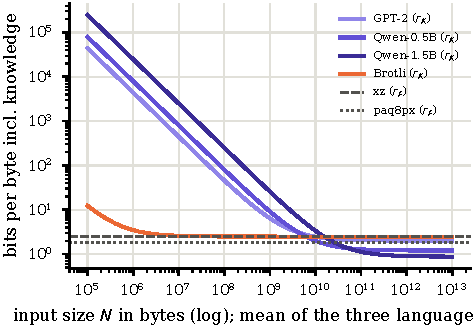
\includegraphics[width=\columnwidth]{breakeven}
\caption{Rate including pretrained knowledge, $r_K(N)$, against input size $N$ (mean of the three language slices). Horizontal lines: self-contained rate of xz and paq8px on the same slices.}
\label{fig:breakeven}
\end{figure}

\subsection{Script and tokeniser}\label{sec:scriptres}
\Cref{tab:tok} splits each language model's payload into tokens per byte and bits per token, and \cref{fig:languages} compares the methods across scripts. On English the two tokenisers produce the same number of tokens (\NumGptEntpb{} and \NumQsEntpb{} per byte), so the whole difference between GPT-2 and Qwen-0.5B (\NumGptEnrP{} vs \NumQsEnrP{}\,bpb) is prediction: \NumGptEnbpt{} against \NumQsEnbpt{} bits per token. On Hindi, GPT-2's tokeniser emits \NumGptHitpb{} tokens per byte against Qwen's \NumQsHitpb{}, while the bits per token are close (\NumGptHibpt{} and \NumQsHibpt{}); on a logarithmic scale the token count accounts for \NumTokShareHi{} of the gap. On Chinese GPT-2 needs \NumGptZhtpb{} tokens per byte against \NumQsZhtpb{}; the token count alone accounts for more than the entire gap (\NumTokShareZh{}), because Qwen's longer tokens each carry more information (\NumQsZhbpt{} bits). Holding the tokeniser fixed, tripling the model from 0.5B to 1.5B parameters lowers the payload by \NumScaleEn{} on English and \NumScaleHi{} on Hindi.

Bits per byte flatter scripts with multi-byte characters. Per character, Qwen-0.5B spends \NumQsEnbpcV{} bits on English, \NumQsHibpcV{} on Hindi and \NumQsZhbpcV{} on Chinese (\cref{tab:tok}); the Leipzig files are not translations of each other, so these figures compare scripts, not languages.

\begin{table}[t]\centering\caption{Language-model payload rate split into tokens per byte (tokeniser) and bits per token (prediction): $r_P=(T/N)(8P/T)$; also bits per character and per line (one sentence per line in the Leipzig files). No piece needed the raw fallback.}\label{tab:tok}\footnotesize\setlength{\tabcolsep}{3.5pt}
\begin{adjustbox}{max width=\columnwidth}\begin{tabular}{@{}llrrrrr@{}}\toprule
Model & Text & Tok./byte & Bits/tok. & $r_P$ & Bits/char & Bits/line\\\midrule
GPT-2 & English & 0.217 & 5.74 & 1.246 & 1.25 & 164\\
GPT-2 & Hindi & 0.596 & 2.59 & 1.542 & 3.90 & 394\\
GPT-2 & Chinese & 0.690 & 4.68 & 3.229 & 8.00 & 329\\
GPT-2 & enwik8 & 0.286 & 4.21 & 1.204 & 1.21 & 103\\
\midrule
Qwen-0.5B & English & 0.219 & 4.95 & 1.083 & 1.08 & 143\\
Qwen-0.5B & Hindi & 0.364 & 2.39 & 0.870 & 2.20 & 222\\
Qwen-0.5B & Chinese & 0.273 & 5.96 & 1.627 & 4.03 & 166\\
Qwen-0.5B & enwik8 & 0.264 & 3.29 & 0.869 & 0.87 & 75\\
\midrule
Qwen-1.5B & English & 0.219 & 4.46 & 0.975 & 0.98 & 129\\
Qwen-1.5B & Hindi & 0.364 & 2.09 & 0.761 & 1.92 & 195\\
\bottomrule\end{tabular}\end{adjustbox}\end{table}

\begin{figure*}[t]\centering
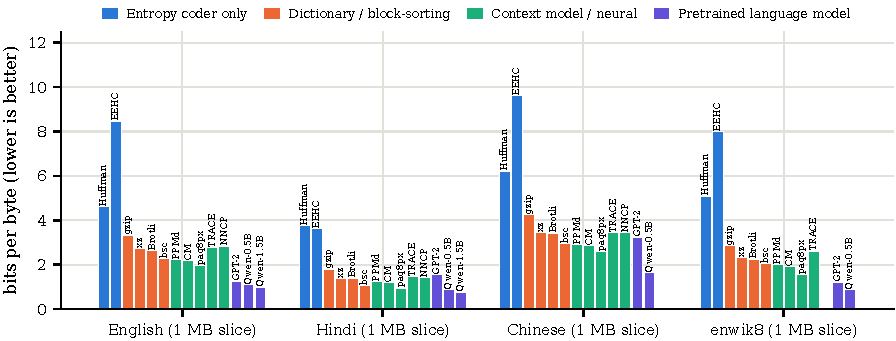
\includegraphics[width=\textwidth]{languages}
\caption{Bits per byte on the 1\,MB slices of English, Hindi, Chinese and enwik8, by method family. Labels name each bar's method.}
\label{fig:languages}
\end{figure*}

\subsection{Huffman-family coders}\label{sec:huff}
Plain order-0 Huffman coding stays within \NumHuffOverHzeroMax\% of the order-0 entropy on every file, and rANS, which is not limited to whole bits per symbol, is \NumRansUnderHuff\% smaller on average (\cref{tab:full}). Rebuilding the tree every 4\,KiB from the bytes seen so far (block-wise dynamic Huffman~\cite{klein2024dynhuff}) costs at most \NumDynOverStaticMax\% against static Huffman and needs no stored table. Coding blocks instead of bytes, as Extended Huffman and EEHC do, helps only when whole blocks repeat: of the \NumEEHCfiles{} full files, EEHC's decodable output is larger than order-0 Huffman's on \NumEEHCworseThanHuffman{}, and only the highly repetitive \texttt{xml} benefits (\NumFEehcXml{} vs \NumFHufXml{}\,bpb). On English sentences EEHC's file is larger than the input (\NumFEehcEn{}\,bpb), even though its payload alone is \NumEEHCpayloadEn{}\,bpb. The base-8 tree adds up to \NumBaseEightMax\% over a binary tree on the same blocks, as expected: a binary Huffman code is optimal in bits, and any base-8 code is a binary code with 3 bits per digit.

\subsection{Speed and memory}
\Cref{fig:speed} places each method by compression speed and mean rate on the slices. The cost of the last bits is steep: zstd and Brotli run at megabytes per second, PPMd and bsc remain fast, zpaq and our CM coder run at hundreds of kilobytes per second, and paq8px, NNCP, TRACE and the language models fall to kilobytes per second in both directions, since every one of them decodes by repeating the encoder's computation. paq8px at level~9 also needs 4.3\,GB of memory, and the language models need a GPU.

\begin{figure}[t]\centering
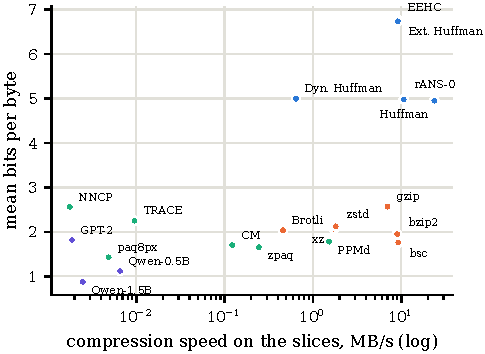
\includegraphics[width=\columnwidth]{speed}
\caption{Compression speed (log scale) against mean bits per byte on the 1\,MB slices. Colours as in \cref{fig:languages}.}
\label{fig:speed}
\end{figure}


\section{Discussion}
\textbf{Which method should one use?} The answer depends on what the decoder already holds. If nothing is shared in advance, the context-mixing compressors (zpaq, paq8px) give the smallest self-contained text files, at kilobytes per second; bsc and PPMd come within 10--15\% of them at megabytes per second; and xz, zstd and Brotli remain the practical choice when decoding speed matters. A pretrained language model is the smallest by a wide margin \emph{if} the decoder already has its weights and a GPU, which is plausible inside a system that runs the same model for other purposes, and implausible for archival or transmission between arbitrary machines. Our break-even sizes make this concrete: the knowledge in even the smallest useful model is repaid only after gigabytes of text.

\textbf{Multilingual fairness is mostly a tokeniser problem.} Haddadi and Teahan found a 1B-parameter LLaMA model far behind classical baselines on non-English text~\cite{haddadi2026comparing}, and Narashiman and Chandrachoodan saw GPT-2 expand Hindi~\cite{narashiman2024alphazip}. Our decomposition attributes the large majority of GPT-2's Hindi deficit, and all of its Chinese deficit, to the number of tokens its English-centred tokeniser produces, consistent with the tokenisation disparities measured by Petrov et al.~\cite{petrov2023tokenizers}. A multilingual tokeniser at a smaller model size (Qwen-0.5B) removes the deficit entirely, and the 1.5B model is then the best compressor we measured on Hindi. For compression, the choice of tokeniser matters more than a tripling of model size.

\textbf{Payload-only reporting misleads most for codebook methods.} EEHC's payload is small because each distinct block receives a short code, but the decoder needs every distinct block, so the codebook grows with the input's diversity. On natural-language text almost every 4-, 8- or 16-byte block is new, and the codebook makes the file larger than the input. The same bookkeeping applies, with different numbers, to DZip's stored bootstrap model and to language-model weights; reporting $r_P$, $r_F$ and $r_K$ side by side removes the ambiguity.

\textbf{Threats to validity.}\label{sec:threats}
(i) Slow methods ran on 1\,MB slices, which favours pretrained models and penalises online learners (TRACE, NNCP), which improve with more data; we state the slice size everywhere. (ii) NNCP ran in CPU mode with its default profile because its CUDA build crashed with our driver, and DZip and TRACE needed small compatibility fixes (listed in the repository); none of the fixes changes the coding. (iii) The largest language models used in prior work (7B and 70B parameters) do not fit our 6\,GB GPU; our models are 0.1--1.5B. (iv) Most runs shared the laptop with other jobs, so the speeds in \cref{fig:speed} are indicative; ratios are exact and every result was decoded and verified. (v) Our Python implementations of dynamic Huffman and rANS are not optimised; their speeds should not be compared with C implementations. (vi) The Leipzig sentence files are not parallel translations; cross-script per-character figures compare scripts and corpora, not languages.


\section{Conclusion}
We measured \NumMethods{} lossless text compressors, from order-0 Huffman coding to 1.5B-parameter language models, in one verified harness on a laptop. Three conclusions hold across English, Hindi and Chinese. First, pretrained language models give by far the smallest payloads (\NumSQlHi{}\,bpb on Hindi, \NumSQlEn{}\,bpb on English), but their weights are repaid only after \NumBreakEvenSmall{}--\NumBreakEvenLarge{} of text against xz, and later against paq8px. Second, when language models fail on non-English text, the tokeniser is usually to blame, not the model. Third, block-codebook Huffman schemes such as EEHC look excellent when only the payload is counted and lose to order-0 Huffman once the codebook is included. We recommend that compression papers report the payload, the self-contained file and the pretrained knowledge separately, and give the break-even input size.

Future work: compressing a language model's weights losslessly, for example with exponent coding as in ZipNN or DFloat11~\cite{hershcovitch2024zipnn,zhang2025dfloat11}, lowers $K$ and therefore $N^\ast$; text-specific tokenisers trained for compression could close the remaining gap for Indic scripts; and larger corpora would let the online neural compressors show their asymptotic behaviour.


\section*{Data and Code Availability}
The harness (\texttt{research/bench}), analysis scripts, corpus-building scripts and raw JSONL logs are in the project repository. The corpora are public: Leipzig Corpora Collection (CC BY), enwik8, Silesia and Canterbury.

\section*{Disclosure}
[Authors: state here, as required by the target venue, how AI-based tools were used in running the experiments and preparing the manuscript.]

\bibliographystyle{IEEEtran}
\bibliography{../common/references}

\end{document}
